176. \begin{figure}[ht!]
\center{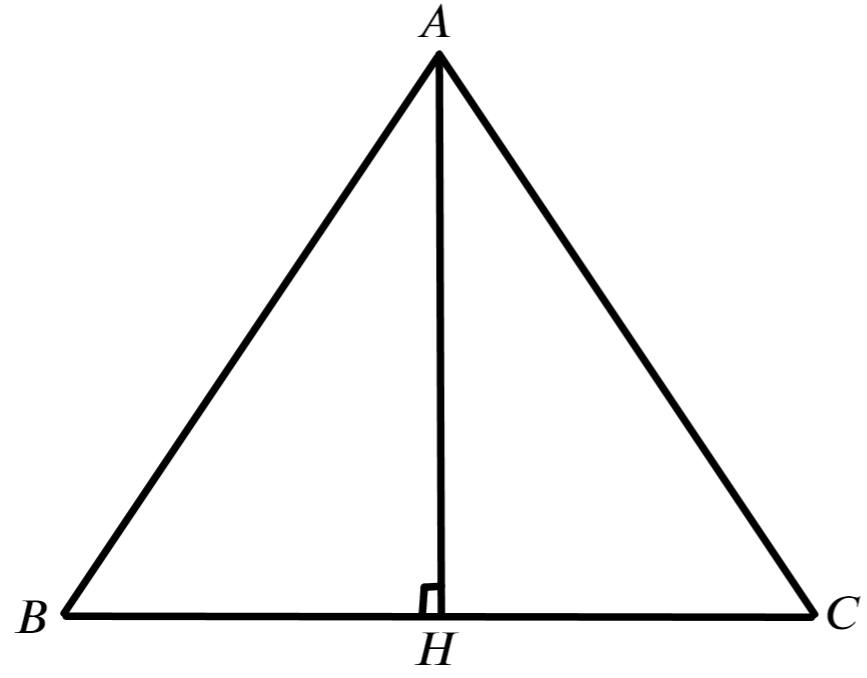
\includegraphics[scale=0.35]{g9-176.png}}
\end{figure}\\
Опустим высоту и медиану $AH,$ тогда $AH=\sqrt{17^2-8^2}=15$ и $S_{\Delta ABC}=\cfrac{1}{2}\cdot16\cdot15=120.$\\
$a)$ Пусть высота из точки $B$ равна $h,$ тогда $S_{\Delta ABC}=\cfrac{1}{2}\cdot17\cdot h=120,$ откуда $h=\cfrac{240}{17}.$\\
$b)$ Пусть радиус вписанной окружности равен $r,$ тогда $S_{\Delta ABC}=rp=r\cdot\cfrac{16+17+17}{2}=r\cdot25=120,$ откуда $r=\cfrac{120}{25}=\cfrac{24}{5}.$\\
$c)$ Пусть радиус описанной окружности равен $R,$ тогда $S_{\Delta ABC}=\cfrac{abc}{4R}=\cfrac{16\cdot17\cdot17}{4R}=120,$ откуда $R=\cfrac{4\cdot17\cdot17}{120}=\cfrac{289}{30}.$\\
